\chapter{Verification and Validation of D3driver}
\label{chap: vod}

This document details the verification and validation of D3driver. In general, verification process is done to check if all the requirements has been incorporated correctly into the product whereas validation process is to get the product tested with the stakeholder/customers to confirm that the product is according to their requirements. In this thesis, the two types of tests are done in the following way:
\begin{enumerate}
\item Verification process based on the \textit{Evaluation Criteria} that was described to screen the existing bots in section \ref{evalcrit}.
\item Validation process based on the conversation simulation between two members of the mechatronics domain. 
\end{enumerate} 

\section{Evaluation criteria - Revisited}

The Evaluation criteria that was described (based on the Requirement characteristics) in Chapter \ref{chap: eoeb} were used to check the suitability of existing bots in the context of employee motivation towards documenting design decisions. In this section, D3driver will go through the same set of criteria to get through the verification process. 

\begin{table}[h]
 \centering
\resizebox{17cm}{!}{%
\begin{tabular}{ll}
\hline
\multicolumn{1}{|c|}{\textbf{Evaluation criteria}} &  \multicolumn{1}{c|}{\textbf{D3driver}} \\ \hline
\multicolumn{1}{|l|}{Workspace - MS teams} & \multicolumn{1}{l|}{Operational in MS teams(prototype)} \\ \hline
\multicolumn{1}{|l|}{Message tagging/labeling(VDI specific)} & \multicolumn{1}{l|}{Provides decision templates in 3 important V-model design phases} \\ \hline
\multicolumn{1}{|l|}{Design decision management} & \multicolumn{1}{l|}{Clearly distinguishes normal conversations from design decisions} \\ \hline
\multicolumn{1}{|l|}{Design decision documentation} & \multicolumn{1}{l|}{Offers a separate tab to view discussed design decisions} \\ \hline
\multicolumn{1}{|l|}{Design decision Knowledge management} & \multicolumn{1}{l|}{Allows members to save a copy of the discussed decisions as PDF} \\ \hline
\multicolumn{1}{|l|}{Easy metadata retrieval} & \multicolumn{1}{l|}{ A workaround to retrieve raw data as JSON is enabled} \\ \hline
                                          
\end{tabular}
}
\captionsetup{justification=centering}
\caption{D3driver against the evaluation criteria
\label{ecr}}
\end{table}

\section{Conversation simulation using D3driver} 
The validation process was done through simulating an ``Engineering Situation" between two stakeholders using D3driver. The end goal of this exercise was to mimic the conversation as if in a product development environment. This helped in establishing helpful user stories to realize D3driver as an effective solution to the problem statement of this thesis.

The agenda of this workshop was as follows
\begin{itemize}
\item Initial setup --- A channel was created in Microsoft teams for the validation purpose. The bot D3driver was added to the channel. The supervisors(members) were also added to the channel. 
\item Stakeholder roles --- The supervisors were defined specific roles to replicate a real scenario. 
\item Design Phases --- The two members discuss some design decisions in each of the V-model phase. The stakeholder roles are re-defined in every phase.
\item Validation --- The members use all the commands and test all the features of D3driver that includes working of ``D3driver messaging extension", ``configurable D3driver tab" , ``search box", ``sort button", ``Export as PDF" button and ``View JSON" button. 
\item At the end of this workshop, the members were also given a survey of questionnaire that was based on the evaluation criteria. 
\end{itemize}

\subsection{User stories}
There are 3  V-model design phases that are taken into account by D3driver to document design decisions hence 3 scenarios are illustrated in this section. The name of the design phase and the roles defined are mentioned for each illustration. There are also member names present in the parenthesis according to their MS teams user IDs. The use case to each phase is also elaborated. To begin with, one of the members initialized the channel by invoking the bot as shown in \ref{fig:initadp}, an appropriate message sent by the bot can also be observed in the screenshot. 


\begin{figure}
\centering
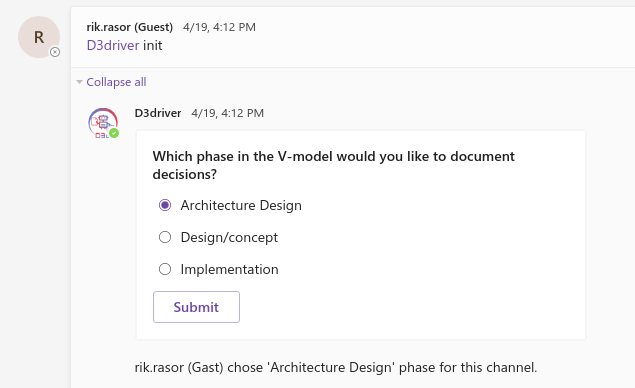
\includegraphics[width=0.7\linewidth]{figures/initadp}
\caption{Channel initialization}
\label{fig:initadp}
\end{figure}


\begin{enumerate}
\item Phase - \textbf{Architecture phase} \newline
Roles - \textbf{Product owner (st.a.pfeifer (Gast))  and Systems architect (rik.rasor (Gast))} \newline
Use case 1 - \textbf{Decision on Logical design} 

In this phase, the two members discuss in short about a logical design decision related to Voltage as shown in \ref{fig:discussionadp}. These conversations are termed as normal messages in the group chat which are of least importance. After a quick initial discussion, the team members choose to document the design decision which they think is significant. Hence, they use D3driver messaging extension to document their decision. When they submit the decision to the group chat, a decision card is posted by D3driver and is depicted in \ref{fig:lddbyd3d}.

\begin{figure}
\centering
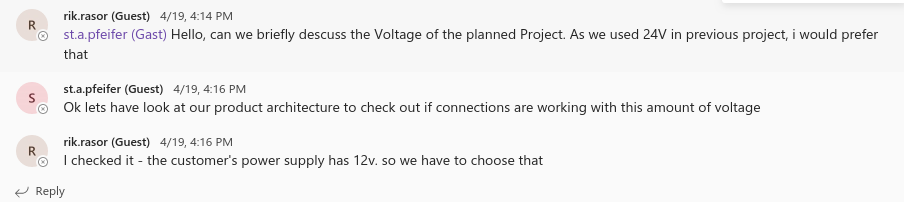
\includegraphics[width=0.8\linewidth]{figures/discussionadp}
\caption{Normal group discussions}
\label{fig:discussionadp}
\end{figure}

\begin{figure}[h]
\centering
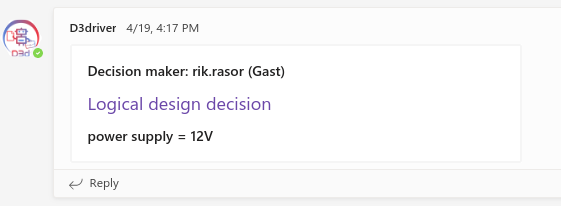
\includegraphics[width=0.7\linewidth]{figures/lddbyd3d}
\caption{Logical design decision card}
\label{fig:lddbyd3d}
\end{figure}

\newpage

Use case 2 - \textbf{Decision on Functional design}

In the subsequent use case, the members had a brief discussion on the functionality of intended device of their planned project. One of the members inquired if the device should be connected to an app or was it sufficient to use the control on the device itself. The other member chose their preference and made a decision and documented it using D3driver as shown in \ref{fig:fddadp}


\begin{figure}[h]
\centering
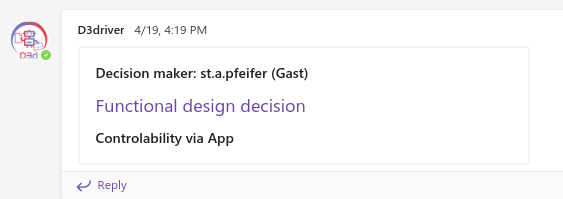
\includegraphics[width=0.8\linewidth]{figures/fddadp}
\caption{Functional design decision card}
\label{fig:fddadp}
\end{figure}

The team members wished to re-initialize the channel with a different V-model phase. Hence, they saved their previous design decisions by clicking on the ``Export as PDF" in D3driver tab as shown in \ref{fig:d3dtabadp}. The downloaded file was also viewed as shown in \ref{fig:pdffile}. They members were also able to view the metadata by clicking on ``View JSON" as shown in \ref{fig:json}. The next step was to use the delete command before re-initialization as shown in \ref{fig:delete}

\begin{figure}[h]
\centering
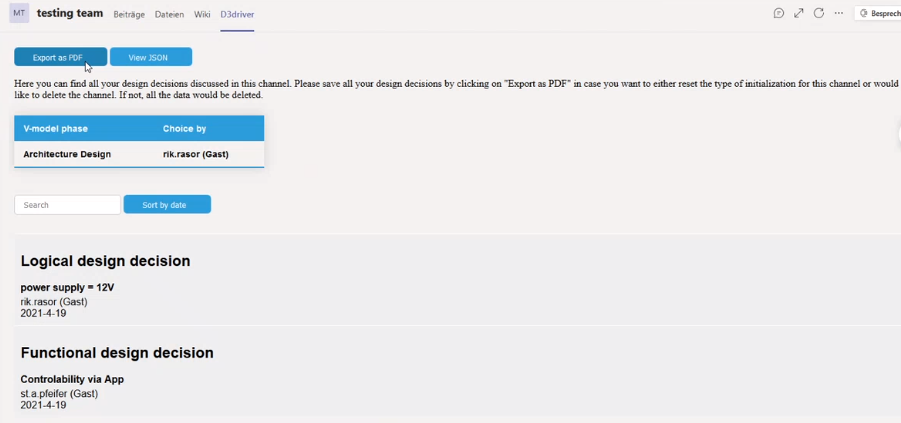
\includegraphics[width=0.8\linewidth]{figures/d3dtabadp}
\caption{D3driver tab features}
\label{fig:d3dtabadp}
\end{figure}

\begin{figure}
\centering
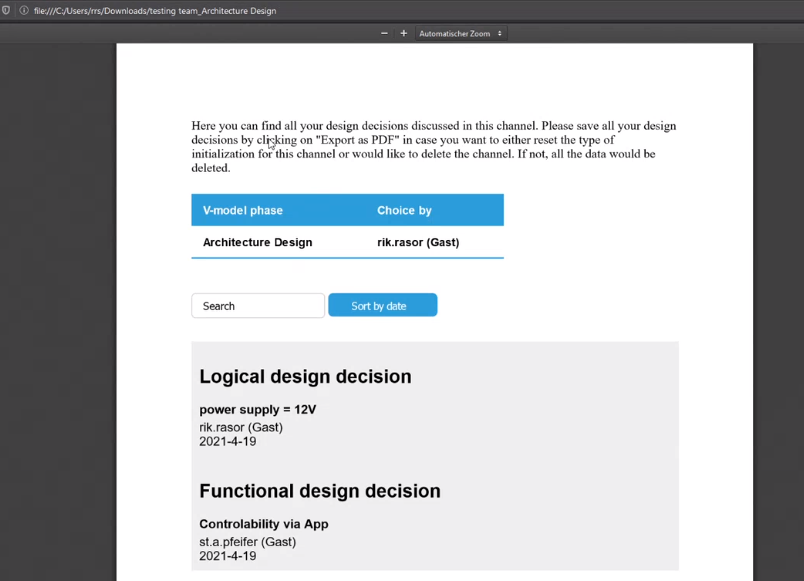
\includegraphics[width=0.7\linewidth]{figures/pdffile}
\caption{View of downloaded PDF file}
\label{fig:pdffile}
\end{figure}


\begin{figure}
\centering
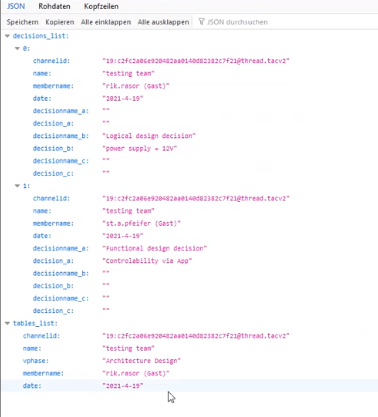
\includegraphics[width=0.7\linewidth]{figures/JSON}
\caption{JSON data view}
\label{fig:json}
\end{figure}

\begin{figure}
\centering
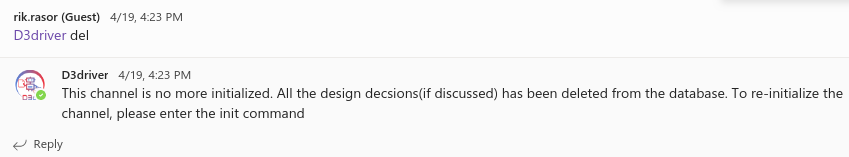
\includegraphics[width=0.8\linewidth]{figures/delete}
\caption{Delete command message}
\label{fig:delete}
\end{figure}



\item Phase - \textbf{Design/Concept phase} \newline
Roles - \textbf{Software Engineer (st.a.pfeifer (Gast) and Mechanical Engineer(rik.rasor(Guest))} \newline
Use case 3 - \textbf{Decision on Design alternatives}

The members once again re-initialize the channel to Design/Concept as shown in \ref{fig:initdc}. The software engineer discusses  control-ability and says that control through software is one option and a motor controller can be implemented so as to regulate the momentum and the velocity of the drives. On the other hand, a mechanical engineer mentions that the control-ability through a clutch is also a good idea. In this scenario, the team members after a discussion arrive at a design decision that they want to document. Hence, they once again use D3driver for decision documentation as shown in \ref{fig:design-alternative-decision}. 

\begin{figure}
\centering
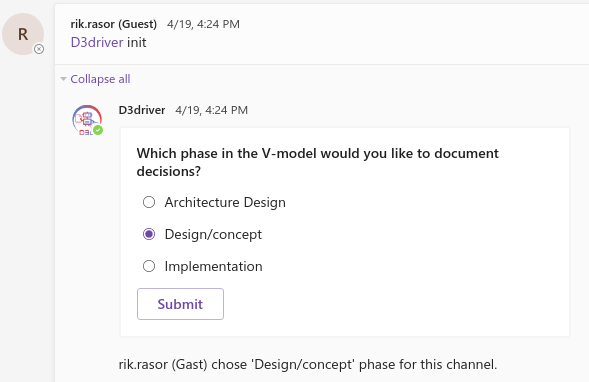
\includegraphics[width=0.7\linewidth]{figures/initDC}
\caption{Re-initialization of channel to Design/concept}
\label{fig:initdc}
\end{figure}


\begin{figure}
\centering
\includegraphics[width=0.7\linewidth]{"figures/design alternative decision"}
\caption{Design alternative decision card}
\label{fig:design-alternative-decision}
\end{figure}



\item Phase - \textbf{Implementation phase} \newline
Roles - \textbf{Two Software engineers (st.a.pfeifer (Gast) and rik.rasor (Gast))} \newline
Use case 4 -  \textbf{Decisions on software design}

At this point, the team saves the discussed decisions, deletes the current initialization and finally re-initializes for the last time as shown in \ref{fig:impleinit} to discuss implementation design decisions. The discussion during the implementation phase is related to the controller parameters. The software implementation of a Proportional–Integral–Derivative (PID) controller for the velocity control of the system was discussed. The two software engineers examine the better values to "P" and finally an experienced decision is made and the team once again uses D3driver to document the software design decision as shown in \ref{fig:software-design-decision}. As a final step, the team also utilizes the search box feature as shown in \ref{fig:search-button}. The sort button was also reviewed and the dates can be sorted in either ascending or descending order as shown in \ref{fig:sort-button}

At this stage, the validation is said to be complete. It can be implied from the user stories and screenshots of the simulation that the D3driver behaves as expected and has proved it's potential to carry out all it's tasks adequately well. The two stakeholders(supervisors) undertook a survey that sought their user experience of D3driver. The survey questionnaire was framed based on the evaluation criteria. Their responses have been recorded and can be viewed here\footnote{https://docs.google.com/forms/d/1U45XPGRnw0L9-CVKsVAX0R-FlWS4dMBfwYolZOzlVZE/viewanalytics} for reference.

\begin{figure}
\centering
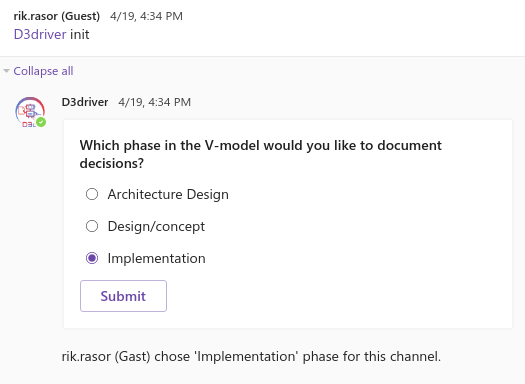
\includegraphics[width=0.7\linewidth]{figures/impleinit}
\caption{Channel initialized to Implementation}
\label{fig:impleinit}
\end{figure}


\begin{figure}
\centering
\includegraphics[width=0.7\linewidth]{"figures/software design decision"}
\caption{Software design decision card}
\label{fig:software-design-decision}
\end{figure}


\begin{figure}
\centering
\includegraphics[width=0.7\linewidth]{"figures/search button"}
\caption{Search box}
\label{fig:search-button}
\end{figure}

\begin{figure}
\centering
\includegraphics[width=0.7\linewidth]{"figures/sort button"}
\caption{Sort button}
\label{fig:sort-button}
\end{figure}

\end{enumerate}




